
\section*{2}

\subsection*{2a}

\begin{figure}[H]
    \centering
    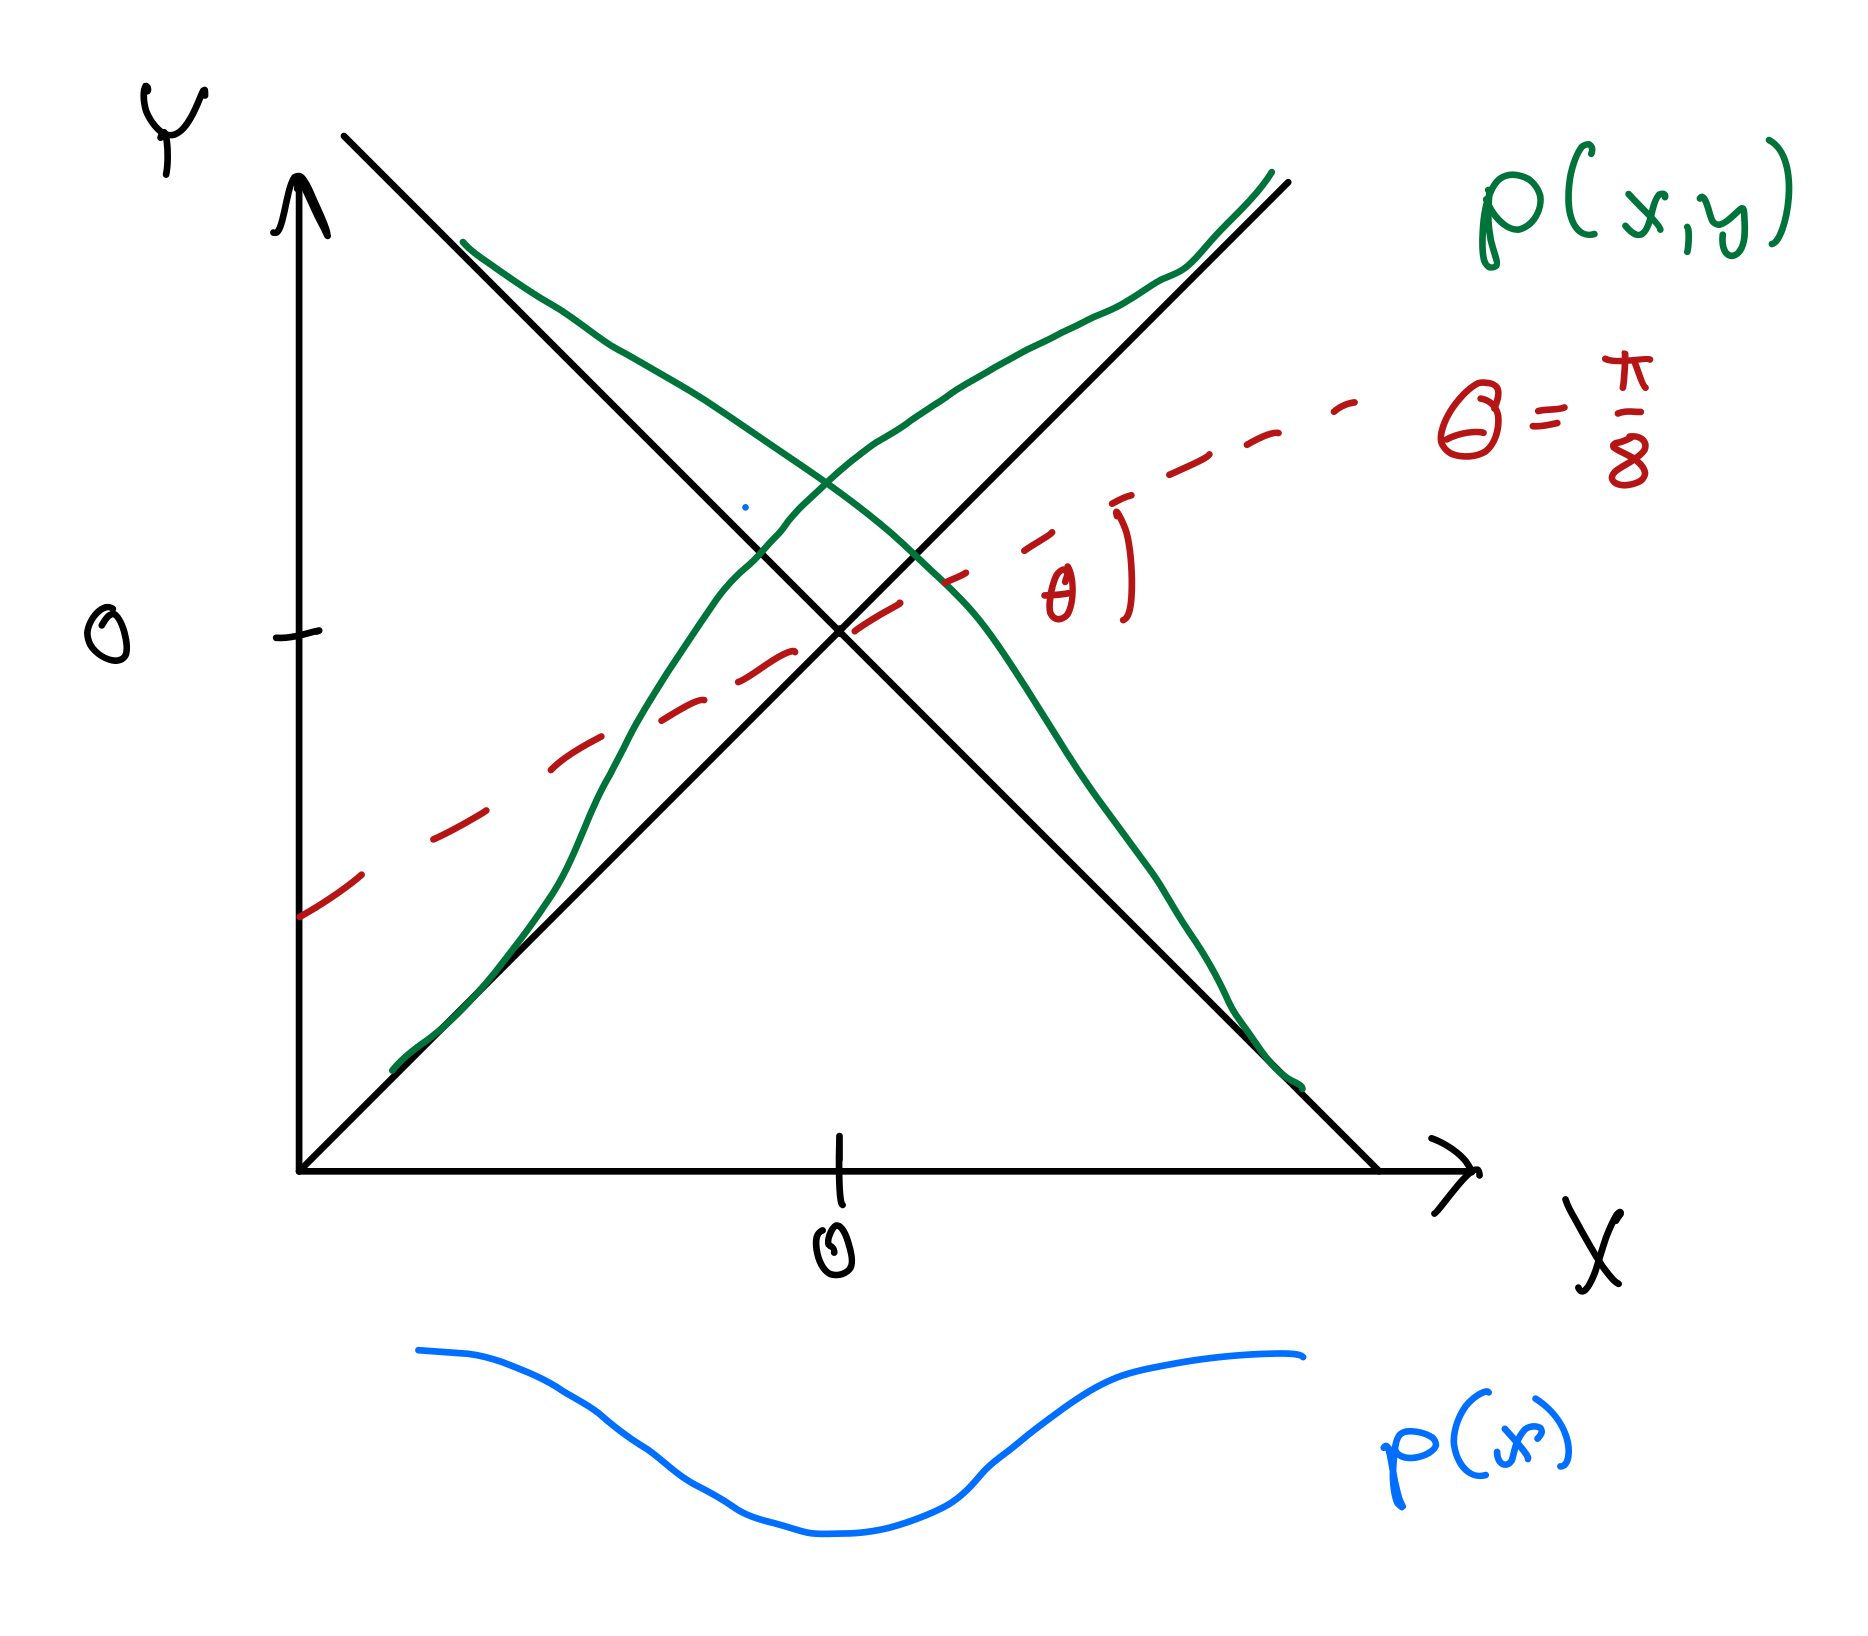
\includegraphics[width=0.8\linewidth]{p_xy.png}
    \caption{Sketch of $p(x, y)$. The black lines indicate where the mass is located and the green
    distributions how the mass is distributed.}
    \label{fig:p_xy}
\end{figure}

\begin{figure}[H]
    \centering
    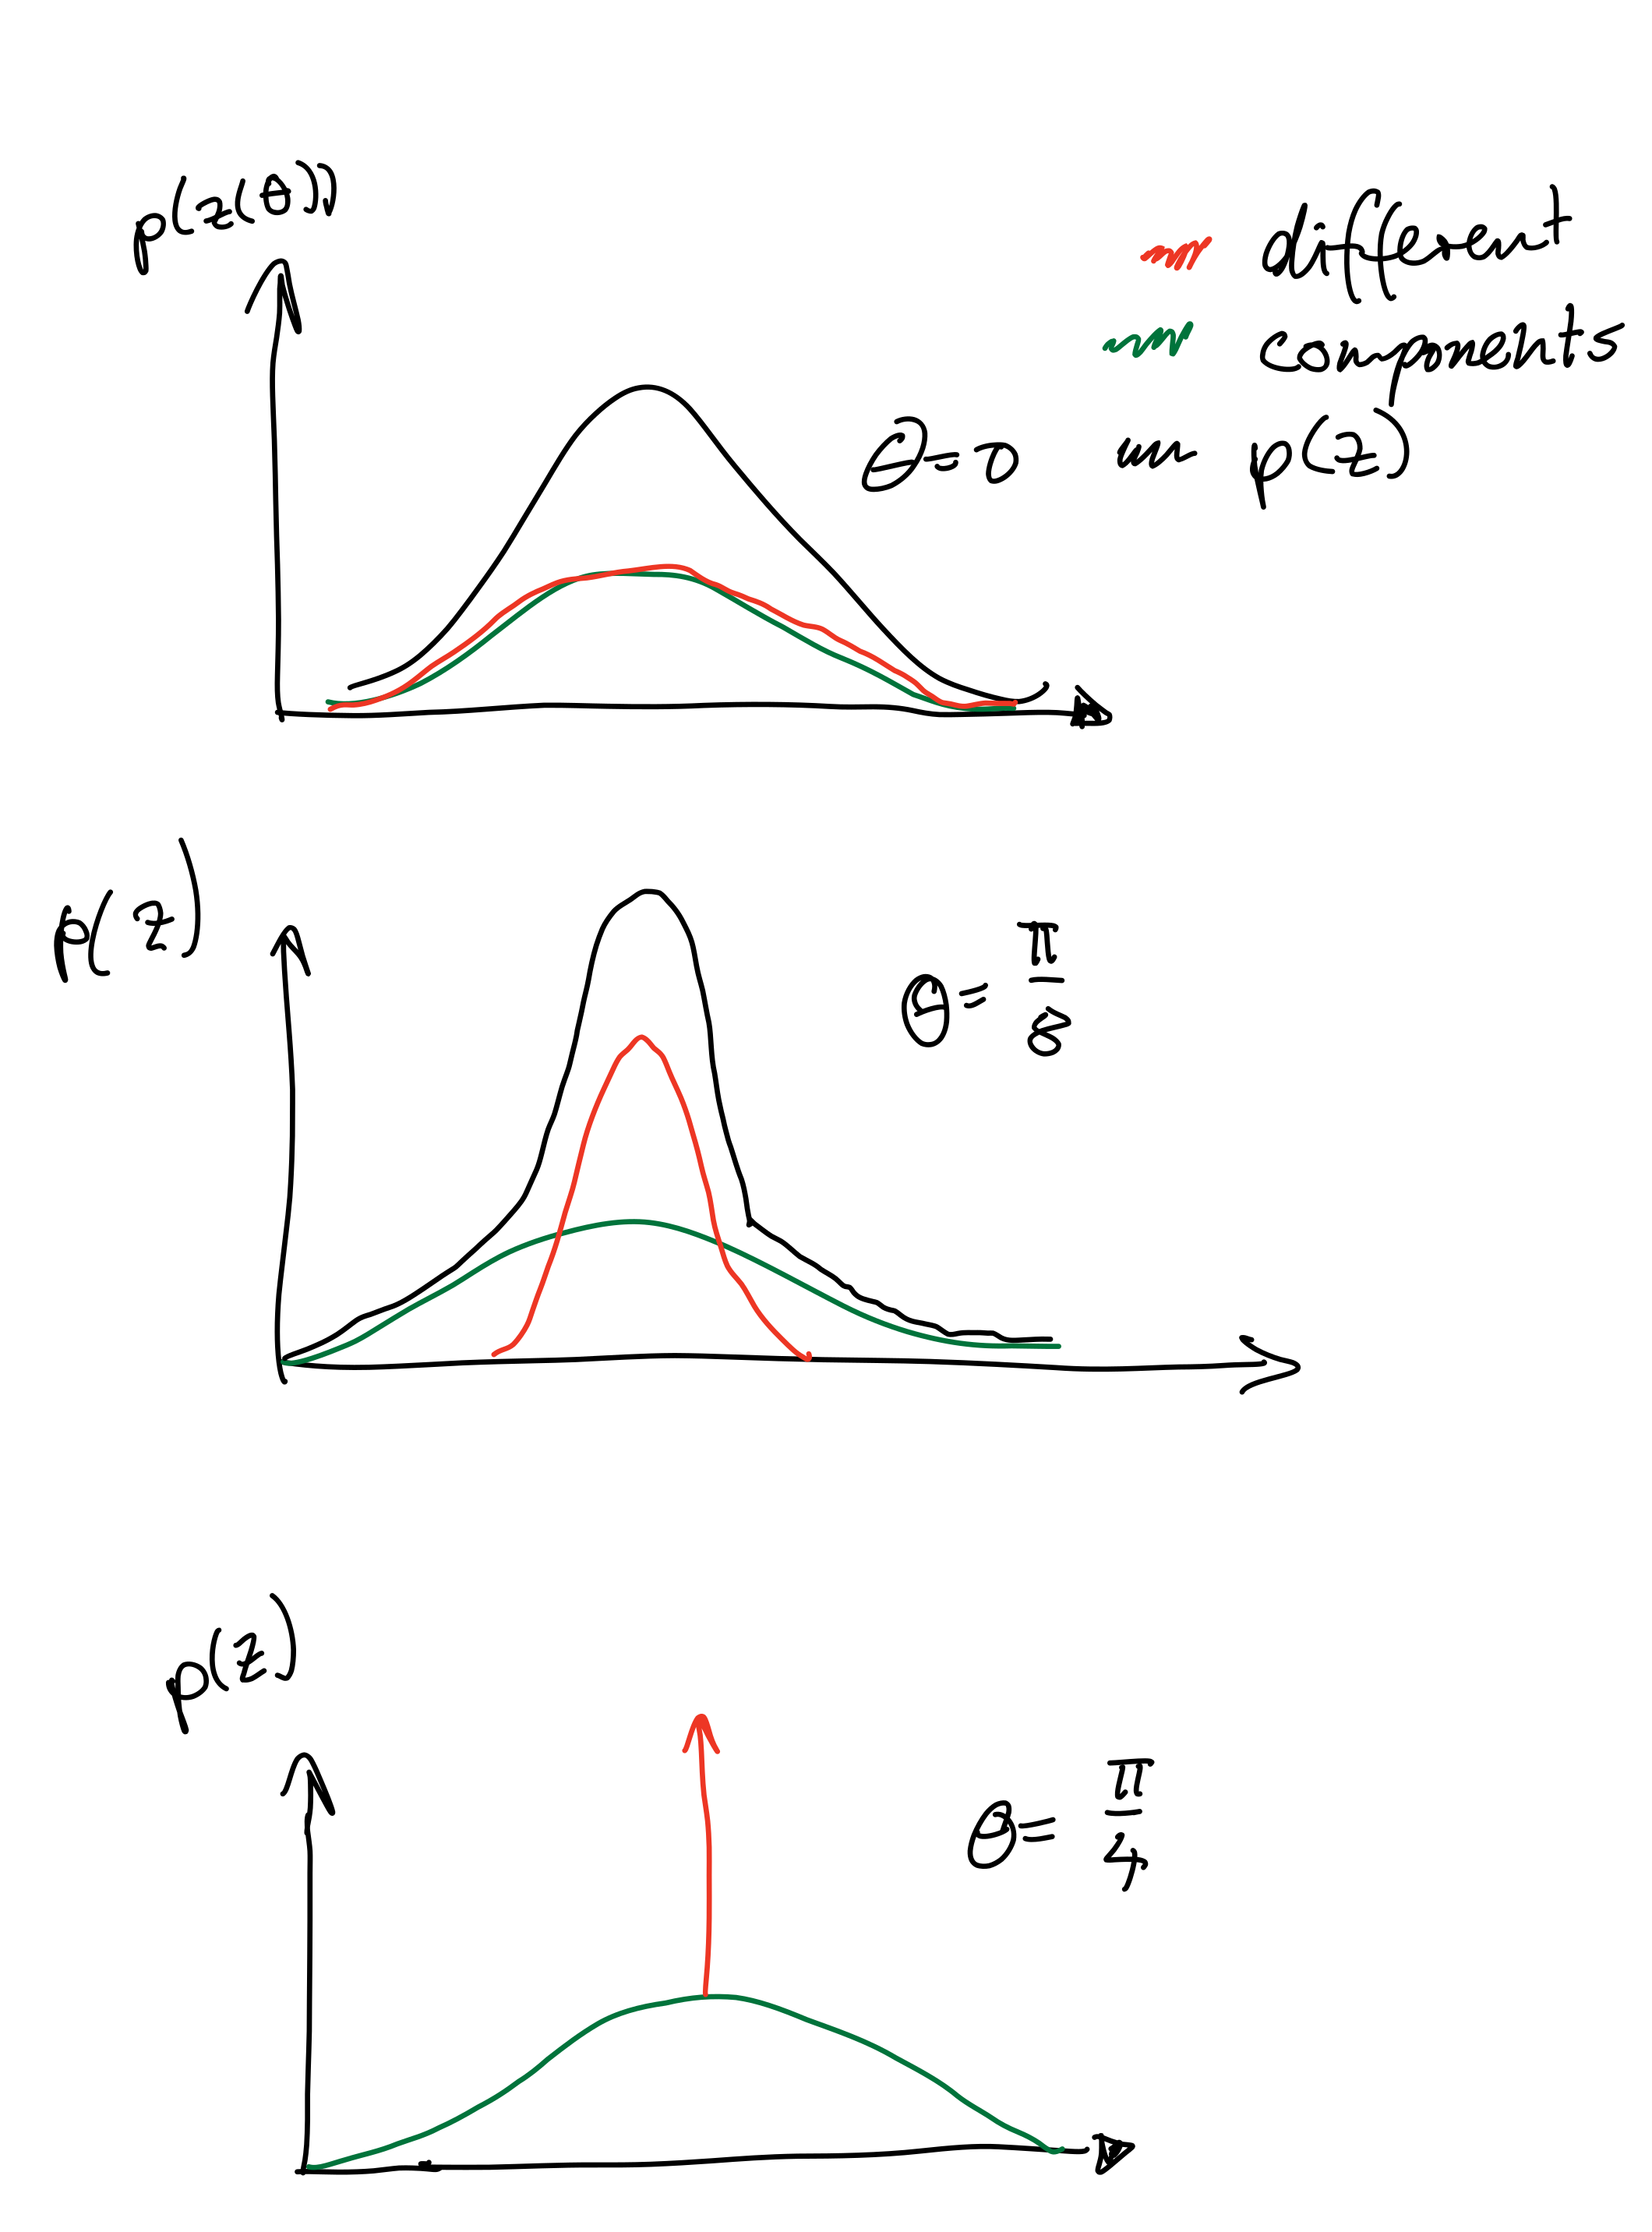
\includegraphics[width=0.8\linewidth]{z_theta.png}
    \caption{$z(\theta)$ for $\theta=0, \theta=\frac{\pi}{8}, \theta=\frac{\pi}{4}$.
    Green and red indicate the different contribution of each of the components.
    The arrow symbolises the dirac delta function.}
    \label{fig:z_theta}
\end{figure}

\subsection*{2b}

As the projection of a gaussian distribution is again a gaussian distribution,
we can write the distribution $p(z(\theta))$ as:
\begin{equation}
    p(z(\theta)) = \frac{1}{2} \mathcal{N}_1(\theta) + \frac{1}{2} \mathcal{N}_2(\theta)
\end{equation}
where $\mathcal{N}_1(\theta)$ is the projection of the distribution of first compontent (the one with angle $\frac{\pi}{4}$)
and $\mathcal{N}_2(\theta)$ analogously for angle $-\frac{\pi}{4}$.

To figure out $p(z(\theta))$, we just have to find the projection of the distribution of both compontents.
The means are 0 and will remain 0 under the projections.
The projection of the simgas are given by:

\begin{align}
    \hat \sigma_1^2 = \left|\cos\left(\theta - \frac{\pi}{4}\right) \right | \\
    \hat \sigma_2^2 = \left|\sin\left(\theta - \frac{\pi}{4}\right) \right |
\end{align}
We ignore the precise intensities in our calculations as only their relative magnitude matter.

Substituting back into $p(z(\theta))$:
\begin{equation}
    p(z(\theta)) = \frac{1}{2} \mathcal{N}_1(0, \hat \sigma_1^2) + \frac{1}{2} \mathcal{N}(0, \hat \sigma_2^2)
\end{equation}

\begin{align}
    \mathbb{V}[Z] &= \int z^2 \left( \frac{1}{2} \mathcal{N}(0, \hat \sigma_1^2) + \frac{1}{2} \mathcal{N}(0, \hat \sigma_2^2) \right) dz = \\
         &= \frac{1}{2} \hat \sigma_1^2 + \frac{1}{2} \hat \sigma_2^2
\end{align}

Now, we want to find the directions that maximizes the variances.
We project the data and therefore $\theta$ and  $\theta - \pi$ result in
the same variance.
Thus we consider only $\cos \left( \theta - \frac{\pi}{4} \right) \ge 0$:
\begin{align}
    \mathbb{V}[Z]= \frac{1}{2} \hat \sigma_1^2 + \frac{1}{2}\hat \sigma_2^2 \\
      \propto \left| \cos \left(\theta - \frac{\pi}{4} \right)\right| + \left| \sin \left(\theta - \frac{\pi}{4} \right) \right| \\
      = \cos \left(\theta - \frac{\pi}{4} \right) + \left| \sin \left(\theta - \frac{\pi}{4} \right) \right| = L
\end{align}
Here, we removed the absolute value around $\cos$, as we know it is always positive.
\def\pif{\frac{\pi}{4}}
For $\theta \ge \pif$:
\begin{align}
    \frac{\partial L}{\partial \theta} & = - \sin\left(\theta - \frac{\pi}{4}\right) + \cos\left(\theta - \frac{\pi}{4}\right) \stackrel{!}{=} 0 \\
                & \iff \cos\left(\theta - \frac{\pi}{4}\right) = \sin\left(\theta - \frac{\pi}{4}\right) \\
                & \iff \theta = \frac{\pi}{2}
\end{align}

For $\theta < \pif$:
\begin{align}
    \frac{\partial L}{\partial \theta} & = - \sin\left(\theta - \frac{\pi}{4}\right) - \cos\left(\theta - \frac{\pi}{4}\right) \stackrel{!}{=} 0 \\
                & \iff - \cos\left(\theta - \frac{\pi}{4}\right) = \sin\left(\theta - \frac{\pi}{4}\right) \\
                & \iff \theta = 0
\end{align}

Therefore, the principal components are $(1, 0)$ and $(0, 1)$ with angles $0$ and $\frac{\pi}{2}$.
\subsection*{2c}

\def\E{{\mathbb{E}}}

\begin{align}
    &\frac{\E[(z(\theta) - \E[z(\theta)])^4]}{\mathbb{V}[z(\theta)]^2} = \\
    & = \frac{\E[z(\theta)^4]}{\mathbb{V}[z(\theta)]^2} \\
    & = \frac{\int z^4 \left(
    \frac{1}{2} \mathcal{N}_1(0, \hat \sigma_1^2) + \frac{1}{2} \mathcal{N}(0, \hat \sigma_2^2) \right) dz
    }{(\frac{1}{2} \hat \sigma_1^2 + \frac{1}{2}\hat \sigma_2^2)^2} \\
    & = \frac{
        \frac{3}{2} \left(\hat \sigma_1^4 + \hat \sigma_2^4\right)
    }{\left(\frac{1}{2} \hat \sigma_1^2 + \frac{1}{2}\hat \sigma_2^2 \right)^2} \\
    & = \frac{\frac{3}{2} \cos(4\theta - \pi)
    }{\left(\frac{1}{2} \left|\cos\left(\theta -\frac{\pi}{4}\right) \right| + \frac{1}{2} \left|\sin\left(\theta -\frac{\pi}{4} \right)\right|\right)^2} \\
    & = \frac{\frac{3}{2} \cos(4\theta - \pi)
    }{\frac{1}{4} + \frac{1}{2}\left|\cos\left(\theta -\frac{\pi}{4}\right) \right| \left|\sin\left(\theta -\frac{\pi}{4} \right)\right|}
\end{align}

Observing that the denominator is minimum for $\pm \frac{\pi}{2}$ and that the
numerator is also maximal for $\pm \frac{\pi}{2}$, yields the two solutions
$\theta = \pm \frac{\pi}{2}$.

